% This is a simple sample document.  For more complicated documents take a look in the exercise tab. Note that everything that comes after a % symbol is treated as comment and ignored when the code is compiled.

\documentclass{article} % \documentclass{} is the first command in any LaTeX code.  It is used to define what kind of document you are creating such as an article or a book, and begins the document preamble
\usepackage{amssymb}
\usepackage{amsmath} % \usepackage is a command that allows you to add functionality to your LaTeX code

\title{Solar crown observation mission study} % Sets article title
\author{Vincent Callegari} % Sets authors name
\date{\today} % Sets date for date compiled
\usepackage{graphicx}
\graphicspath{{./images/graph/}}
% The preamble ends with the command \begin{document}
	\begin{document}
		\maketitle
		\section{introduction}%flemme de faire cette partie pour l'instant
		\section{observation zone}
		\subsection{computing the position of the observation zone}
		
		At first for simplify things we will first consider that the sun and the occulting body are aligned along the X axis.
		
		\begin{figure}[h]
			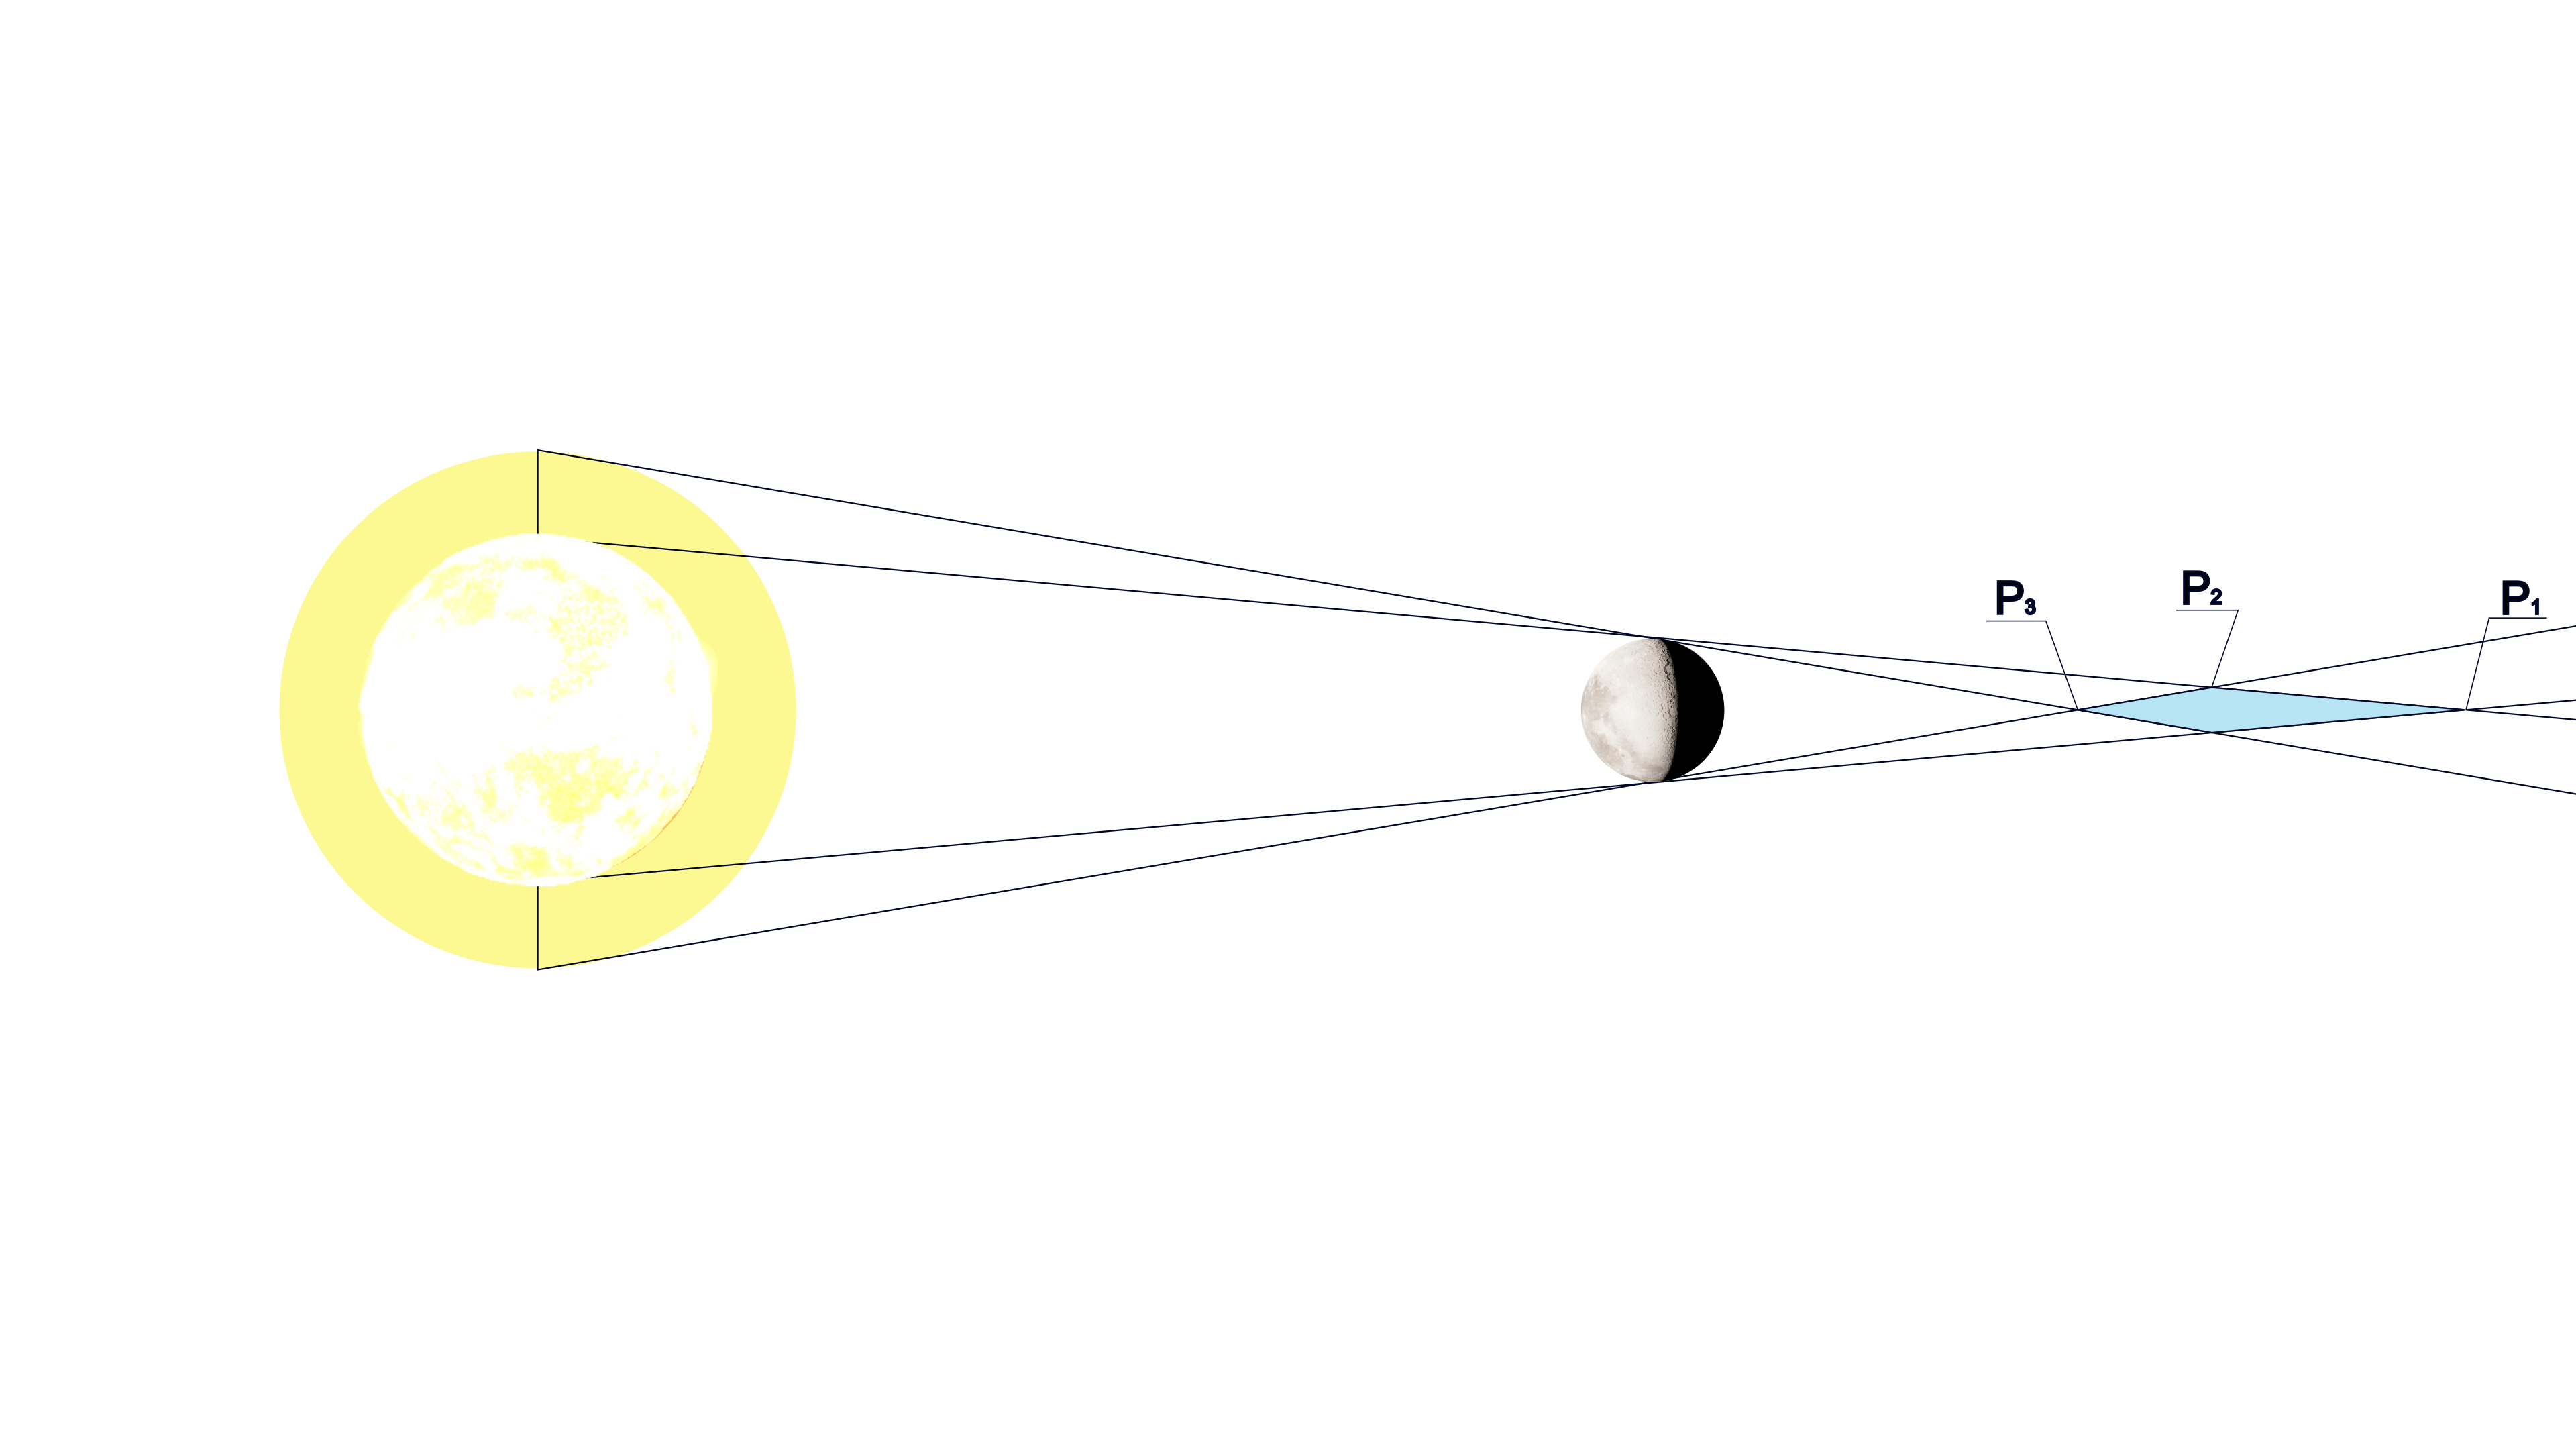
\includegraphics[width=10cm]{images/moon_schem.png}
			\caption{major points of the observation zone }}
		\end{figure}
			
		%durant l'étude de ces problèmes, on se place dans %le référentiel de la Terre avec des coordonnées %cartésienne, l'axe Terre-Soleil étant l'axe X avec
		%l'axe Y colinéaire au plan écliptique de la Terre. 
		
		A point is in the observation zone if the sun is totally hidden and the crown is visible around the occulting body. This zone has the shape of a double cone that we can represent by the rotation of a triangle.
		
		%un point est dans la zone d'observation quand le %soleil est totalement masqué et que la couronne %est visible autour de l'astre occultant. Cette %zone à la forme d'un double cône que l'on peut %représenter comme la rotation d'un losange %mettre un schéma pour être plus clair.
		
		The triangle could be defined by its three points
		$P_1$,$P_2$ et $P_3$, with as coordinates $(P_{1x},0,0)$ , $(P_{2x},P_{2y},0)$,$(P_{3x},0,0)$ 
		
		%le losange peut être définit par 3 points %$P_1$,$P_2$ et $P_3$, ayant pour coordonnée %$(P_{1x},0)$ , $(P_{2x},P_{2y})$,$(P_{3x},0)$ avec %$\hat{x}$ le long de l'axe lune soleil.
		
		The value of $P_{1x}$ and $P_{3x}$ can be easily computed using the Thales theorem.
		
		%les valeurs de $P_{1x}$ et $P_{3x}$ peuvent être %facilement calculée en utilisant le théorème de %Thalès :
		
		$$	
		P_{1x}=\frac{\bar{D}R_l}{R_s-R_l}
		$$ 
		$$	
		P_{3x}=\frac{\bar{D}R_l}{R_s(\alpha+1)-R_l}
		$$
		
		Where $\bar{D}$ is the Solar-Moon distance, $R_s$ the Solar Radius ,$R_l$ the Lunar radius and $\alpha$ is the solar crown's added size in solar radius (the more $alpha$ is near of zero the more the solar crown's radius is near of the solar radius meaning that we will observe part of the crown near of the solar surface)
		%où $\bar{D}$ est la distance Soleil-lune, $R_s$ le rayon solaire ,$R_l$ le rayon lunaire et $\alpha$ est la taille supplémentaire de la couronne solaire par rapport au rayon solaire( plus $alpha$ est proche de 0 plus on observera des parties de la couronne proche de la surface du soleil).
		
		We can then compute the position of $P_2$ by computing the intersection of the lines linking the surface of the Moon and the points $P_1$ and $P_3$
		
		%on peut ensuite calculer la position de $P_2$ en calculant l'intersection des lignes reliant la surface de la Lune au points $P_1$ et $P_3$ : 
		
		$$
		P_{2x}=\frac{P_{1x}tan(\theta_1) + P_{3x}tan(\theta_3)}{tan(\theta_1) + tan(\theta_3)}
		$$
		$$
		P_{2y}=tan(\theta_1)(P_{1x}-P_{2x})
		$$
		
		with
		$$
		\theta_1=\sin^{-1}\left(\frac{R_l}{P_{1x}}\right)
		$$
		
		$$
		\theta_3=\sin^{-1}\left(\frac{R_l}{P_{3x}}\right)
		$$
		
		with $\alpha=0.05$
		
		\subsection{approximation of the zone}
		
		We could use directly the result obtained earlier in the simulation but as checking if the device is in the observation zone will be one of the most reapeated computing of the code i think it is usefull to look for approximation that could reduce computing.
		
		The Position of the points $P_1$,$P_2$ and $P_3$ relative to the moon will change depending of the moon position around the earth, hovewer the shape of the the zone in itself will not change much (with a dimension error smaller than 0.5\%)
		
		%la position des points $P_1$,$P_2$ et $P_3$ par rapport à la Lune vont changer en fonction de sa position autour de la Terre. Cependant la forme de la zone en elle même varie assez peu (les dimensions variant de moins de 0.5\%).
		
		We can obtain a good approximation of the observation zone at any position of the moon around the Earth by computing the shape of the observation zone with the moon at the origin and then move it and rotate it to place it at the right position.
		%On peut donc obtenir une bonne approximation de la zone d'observation où que se trouve la Lune autours de la Terre en calculant la forme de la zone d'observation lorsque la Lune se trouve à la place de la Terre puis de la déformer pour se positionner là où se trouve la Lune.
		
		
		
		We name $\hat{P_1}$, $\hat{P_2}$ and $\hat{P_3}$ the points of the observation zone when the moon is at the origin (which is fixed at the average distance between the Earth and Sun $D$). the points $P_1$ and $P_3$ are collinear with the vector $R_{ls}$ witch are the position of the Moon relative to the Sun.
		
		As the value of $P_1$ and $P_3$ are proportional to the distance between the Moon and Sun 
		
		Also we take the points $\hat{P_1}$ $\hat{P_3}$ so they are colinear with the X axis. We can conclude of the following formula of the points $P_3$ and $P_1$.
		
		%On nomme $\hat{P_1}$, $\hat{P_2}$ et $\hat{P_3}$ les points de la zone d'observation quand la Lune est à la place de La Terre. Les points $P_1$ et $P_3$ sont colinéaire avec le vecteur $R_{ls}$ qui représente la position de la Lune par rapport au Soleil.
		%De plus les points $\hat{P_1}$ $\hat{P_3}$ sont colinéaire avec l'axe X. On peut en déduire les formules suivantes de la position de $P_3$:
		
		$$
		\begin{equation}
			P_3=R_{lt}+\hat{P_{3x}}D^{-1}R_{ls} 
		\end{equation}
		$$
		$$
		\begin{equation}
			P_1=R_{lt}+\hat{P_{1x}}D^{-1}R_{ls} 
		\end{equation}
		$$
		
		%vérifier si un point $S$ est dans la zone d'observation revient à vérifier les inégalités suivantes:
		A point $S$ is considered in the observation zone if the following inequality are verified : 
		
		$$
		\begin{equation}
			\begin{align}
				||a||&<||b||p_1\\
				||a||&<O-||b||p_2\\
				||S||&>||P_3||
			\end{align}	
		\end{equation}
		$$
		
		
		with $b$ being the projection of $S-P_3$ on the axis Sun-Moon, $a=S-P_3-b$. $p_1$, $p_2$ and $O$ are real value: here this parameter will be approximated by their value when the Moon is at the origin :
		
		%avec $b$ la projection de $S-P_3$ sur l'axe Lune- Soleil, $a=S-P_3-b$ et $p_1$, $p_2$ et $O$ sont des réel à déterminer. On remarque que si la Lune est à l'origine on a
		
		$$
		\begin{align}
			p_1&=\frac{\hat{P_2y}}{\hat{P_2x}-\hat{P_3x}}\\
			p_2&=\frac{\hat{P_2y}}{\hat{P_1x}-\hat{P_2x}}\\
			O&=\hat{P_2y}+(\hat{P_2x}-\hat{P_3x})p_2
		\end{align}	
		$$ 
		
		Note that the last condition was added just to avoid a symetric virtual zone that will appear before the $P_3$ point because of the symetry of the norm function.
		
		%En supposant que la forme de la zone d'observation varie peu lorsque la lune se déplace, on peut utiliser les même coefficients où que se trouve la Lune.
		
		%Si on souhaite avoir une approximation un peu plus précise on peu prendre en compte la variation la plus importante sur la forme de la zone d'observation étant la variation de la longueur de la zone.
		
		If we want to increase the precision of the observation zone we can take in account the variation in length of the observation zone by scaling the parameter $b$ by
		
		%On peut prendre en compte cette variation en multipliant $b$ par
		
		$\frac{||\hat{P_1}-\hat{P_3}||}{||P_1-P_3||}$
		
		This approximation is quite precise because the real equation of the point $P_1$,$P_{2x}$ and $P_3$ are linea, meaning there is an error only on the position of $P_{2y}$.
		
		\subsection{numeric application}
		We have the following distances : 
		$$
		\begin{align}
			R_l&=1.7374\times10^6 m \\
			R_s&=6.955\times10^8 m \\ 
			D_{sl}&=1.496\times10^{11} m \\
			\Delta_D=2D_{el}&= 7.69496\times10^8 m
		\end{align}
		$$
		
		We get the following value for the point of the Zone for $\alpha=0.05$ with the moon at the origin
		%on obtient les valeur suivantes pour les points de la zone pour $\alpha=0.05$
		
		$$
		\begin{align}
			P_{3x}&=3.577\times10^8 m \\
			P_{1x}&=3.758\times10^8 m \\ 
			P_{1x}-P_{3x}&=1.7928\times10^7 m \\ 
			P_{2x}&=3.655\times10^8 m \\
			P_{2y}&= 4.248\times10^4 m
		\end{align}
		$$
		
		And here is the variation of these distance when value 
		
		$$
		\begin{align}
			\Delta_{P_{3x}}&=1.835\times10^6 m \\
			\Delta_{P_{1x}}&=1.927\times10^6 m \\ 
			\Delta_{P_{1x}-P_{3x}}&=9.198\times10^4 m \\ 
			\Delta_{P_{2x}-P_{3x}}&=4.487\times10^4 m \\ 
			\Delta_{P_{2x}}&=1.880\times10^6 m \\
			\Delta_{P_{2y}}&= 4.935\times10^{-3} m
		\end{align}
		$$
		
		
		We can see that by using the approximation defined earlier, we are neglecting variation of order lower than thousand of killometer ($10^6 m$).If we add the optimisation on the value of $b$ we are now neglecting variation of order lower than ten killometerss ($10^4 m$) leaving only error of a couple killometers on the  posisiton of $P_{2x}$ which is not a lot against the size of the observation zone : (around $ 20000 km $ by $100 km$).
		
		About the error on $P_{2y}$ the error is of the order of a millimeter and can clearly be neglected.
		
		%on observe qu'en utilisant l'approximation définie plus tôt, on néglige les variation de l'ordre du millier de kilomètres ($10^6 m$). et en ajoutant l'optimisation supplémentaire sur la valeur de $b$ on néglige également les variation de l'ordre de la dizaine de kilomètre ($10^4 m$) ne laissant que les erreurs de l'ordre de quelques kilomètre sur la position de $P_2x$ ce qui ne change pas grand chose compte tenu de la grande longueur de la zone par rapport à son épaisseur (environ $ 20000 km $ contre $100 km$)
		
		%la position de la zone d'observation va se déplacer avec la lune mais va aussi changer de direction et de forme.
		
		%on a $\bar{D}=\sqrt{D^2+2DX_l+r_l^2}$ où $D$ est la distance Terre-Soleil et $R_l=(X_l,Y_l,Z_l)$,$||R_l||=r_l$ la position de la lune relativement à la Terre. $||r_l||<<D$ donc on peut considérer que $\bar{D} \approx \sqrt{D(D+2X_l)}$
		
		%cette approximation crée une erreur sur les position de $X_1$ et $X_3$ de l'ordre $1000m$.
		
		%en prenant une valeur encore plus simplifié de $\bar{D}$ : $\bar{D}=D$ on obtient une erreur sur les positions de  $X_1$ et $X_3$ de l'ordre de $1000km$ mais on conserve une erreur assez faible sur la distance entre $X_1$ et $X_3$ (environ 0.25\% de la distance $X_1$$X_3$ ). Cela permet de considérer la zone d'observation comma ayant toujours la même forme (longueur et épaisseur).
		
		\newpage
		\section{Observation analysis}
		
		\subsection{definition of the problem}
		
		The problem is describe as follow :
		\\
		The Earth Moon Sun system is simulated with the Sun being fixed at the origin. The Coordinate system is then centered without rotating it at the Earth Moon barycenter. The motion of the device is computed by taking in accoun the gravitional pull of the Earth an Moon but we don't apply the force of gravity of the sun, this mean that the device will experience the gravity of the sun as if it wa at the altitude of the Earth-Moon barycenter.This won't make a huge difference considering that the device will stay between 2 Moon-Earth distance from Earth. the trajectory of Earth and Moon will be precompute before running any optimisation algorithm.
		
		The initial position of the Earth and Moon that will be use in this article are their position in January 1st midnight, 2025. their position are retrieved on the horyzon system of Nasa : https://ssd.jpl.nasa.gov/horizons/app.html
		
		%la lune suit une orbite circulaire autour de la Terre de rayon $a=384000km$.
		
		%la forme de la zone d'observation de la Lune est considérée comme étant égale à la zone d'observation de la lune si elle se trouvait à l'origine (la position de la terre). La position du point $P_3$ est déterminé par la formule suivante:
		
		We consider the position and shape of the observation using the formula and approximation defined earlier, with the initial value of the observation zone being computed if the moon was at the origin at time t0.
		this give the following equation :
		$$
		P_3(R_l)=R_{l}+\hat{P_{3x}}D^{-1}R_{ls}
		$$
		with $\hat{P_3}$ being the position of the point $P_3$ when the moon is at the origin
		,$R_{l}$ being the Moon position.
		and $R_{ls}$ is the position of the Moon relatively to the sun.
		
		the objectif is to find trajectory that allow repeated and long observations.
		
		%le but est de trouver des orbites Kepleriennes qui effectue des observations répété et les plus longues possibles.
		
		after testing some possible orbit configuration for the device, it look like most of the observation last only a few minutes, but some precise configuration that we will discuss later can last for multiples hour. This space of solutions suggest that it is better to optimize only one observations that will last longer instead of trying to find trajectory that will make multiples observations but very short ones.
		
		
		
		%Les temps d'observation peuvent beaucoup varier allant d'une durée de quelques minutes à plusieurs heures.	dans la suite on va donc se concentrer sur une seule observation.
		
		%afin de pouvoir reproduire les observations, il vaut mieux prendre une période d'orbite qui est un multiple de celle de la Lune.
		
		in order to make multiple observation, it may be better to take orbital period that are multiple of the moon's, this way the Moon and thus the observation zone would be at the same place when the device get to the observation zone again.
		
		%Hovewer choosing period between the moon orbital period or its synodic period could up to debate.
		hovewer considering that the Sun is moving, it may be better to make the device orbital period equal to the Moon's synodic period but i haven't make enough comparative data to know which one is the best.	
		
		from this we can conclude the following formula for the semi major axis of the device.
		$$
		a_s=a_lk^{\frac{2}{3}}\left(\frac{\mu_t}{\mu_t+\mu_l}\right)^\frac{1}{3}
		$$
		
		with
		$$
		P_s=kP_l
		$$
		
		considering that the objective is to make observation, it seem logical that the device will be in the observation zone at one time or another. This is why i've decided to define the device initial position to be inside the observation zone. In addition the fact that the observation zone is almost flat (around $100$ times longer than thick), we can consider the starting position of the device to be on the segment $[P_3,P_1]$. We will also need a initial time $t_0$ to know when the device cross this segment.
		
		this mean that we can defined the initial position of the device with the following function
		$$
		r_0(t,\lambda)=P_3(t)\lambda+(1-\lambda)P_1(t)
		$$
		
		where $P_3$ and $P_1$ are computed using the Moon position and the formula that we show earlier.
		
		
		
		%étant donné que l'objectif est de faire une observation, on peut faire partir le satellite directement de la zone d'observation.
		
		%De plus la dimension de la zone étant très étirée (environ $10000km\times100km\times100km$) on peut considérer que le satellite coupera forcement le segment $[P_3,P_1]$, on peut donc décrire la position initiale du satellite à l'aide de l'anomalie vraie de la lune $\nu$ et un scalaire $\lambda$ entre 0 et 1. la position initiale du satellite devient : 
		%$$
		%S_0=\lambda(P_1-P_3)+P_3(R_l(\nu))
		%$$
		
		as we have fixed the semi major axis of the device wa can conclude its speed using this formula :
		
		$$
		||\dot{r}(0)||=\sqrt{\frac{2\mu}{||S_0||}-\frac{\mu}{a_s}}
		$$
		
		
		we then just have to choose the direction of the speed vector $\dot{r}_0$ using two angle $\theta_s$ and $\phi_s$.
		
		%on peut ensuite determiner l'orientation de la vitesse initiale avec deux angles $\theta_s$ et $\phi_s$.
		
		%la dynamique du satellite et de la lune doivent être calculé pour calculer le temps de l'observation.
		
		%on à la dynamique suivante :
		
		we must compile the dynamics of the device in order to get the observation time. Here's the dynamics : 
		
		$$
		\begin{bmatrix}
			\dot{\overrightarrow{R_{s}}}\\
			\dot{\overrightarrow{V_{s}}}\\
		\end{bmatrix} =\begin{bmatrix}
			\overrightarrow{V_{s}}\\
			\frac{-\mu_l }{||R_{s}-R_{l} ||^{3}}(\overrightarrow{R_{s}}-\overrightarrow{R_{l}}) + \frac{-\mu_t }{||R_{s}-R_{t} ||^{3}}(\overrightarrow{R_{s}}-\overrightarrow{R_{t}})\\
		\end{bmatrix}
		$$
		
		%avec comme condition initiale :
		with as initial condition
		
		$$
		\begin{bmatrix}
			\overrightarrow{R_{0}}\\
			\overrightarrow{V_{0}}\\
		\end{bmatrix} =\begin{bmatrix}
			\lambda \left(\widehat{P_{1}} -\widehat{P_{3}}\right) +R_{lt} +\frac{\widehat{P_{3x}}}{D} R_{ls}\\
			\sqrt{\mu \left(\frac{2}{||R_{0} ||} -\frac{1}{a_s}\right)}\widehat{v_{0}}( \theta _{s} ,\phi _{s})\\
		\end{bmatrix}
		$$
		
		the differential equation must be solve before and after the initial time $t_0$ to get the time when the device exit and enter the observation zone.
		%la dynamique devra être simulée après et avant l'état initial pour trouver l'instant où l'objet entre et sort de la zone.
		
		%la fonctions d'objectif est définit comme suit :
		the payoff function that will be used to evaluate the interest of one observation is defined as follow
		
		$$
		\int_{-\tau_d}^{\tau_u}dx=\tau_d+\tau_u
		$$
		
		%où $\tau_d$ est l'instant où l'objet rentre dans la zone d'observation et $\tau_u$ l'instant où l'objet en sort.
		
		where  $\tau_d$ and $\tau_u$ are the time when the device enter and exit the observation zone.
		
		we will use the equation (2) to evaluate if the device is in the observation zone at a time $t$.
		
		%l'équation utilisé pour vérifier si l'objet est dans la zone est l'équation (2).
		
		%les paramètre de contrôle sont :
		
		to conclude we have the following variables : 
		
		\begin{itemize}
			\item the initial time $\t_0$ that is used to determine intial position of the observation zone and bodies of the system.%qui définit la position de la zone d'observation.
			\item the initial position within the observation zone $\lambda$ %de l'objet dans la zone d'observation qui est simplifier par un segment allant de $P_3$ à $P_1$. 
			\item the angles $\theta_s$ et $\phi_s$ that defined the intial direction of the object speed.% qui définissent l'orientation de la vitesse de l'objet.
		\end{itemize}
		
		on a donc un espace de dimension 4 :
		$(\nu,\lambda,\theta_s,\phi_s)=[0,2\pi]\times[0,1]\times[0,2\pi]\times[0,\pi]$
		
		l'espace est contraint mais étant donné que la plupart des dimension sont des angles et qu'il suffit de donner un score de 0 si $\lambda$ est en dehors du domaine on peut considéré que l'espace est égal à $\mathbb{R}^4$ pour avoir un problème sans contrainte.
		
		\section{Result}
			
		When we are working with a simple 2D problem with circular Moon orbit , there are an optimum near the value $(2\pi/3,0.5,38/45\pi,0)$ that give observation time of almost 20h.
		
		We managed to get observation time this long because the speed of the object and the observation Zone are equivalent. Meaning that the device can stay in the observation zone for a long time. As the Observation Zone velocity are nearly the same as the Moon, we can simplify for now by saying that the device must have the same speed as the Moon.
		
		The satellite describe a loop inside the observation zone, meaning that it is possible to get two fairly long observation very near to each other if the tip of the loop is outside of the observation zone. ascending if there is a good chance that these solutions are less efficient that a solution with the entire loop inside the observation zone, it could be usefull to improve the objective function to detect when the object reenter the observation zone after a short time.
		
		For the model implemented, i've intentionally kept high value of $\alpha$ to ensure that the loop stayed in the observation zone.		
		
		we can easily determine that there are two point in the lunar orbit where we can obtain very long observation time:
		
		The satellite can have the same speed vector as the moon only if the following equation is verified : 
		
		$$
		\sqrt{\frac{2\mu}{R_s}-\frac{\mu}{a_s}}&=\sqrt{\frac{2\mu}{R_l}-\frac{\mu}{a_l}}
		$$
		
		Considering that the moon's speed is constant (because of its small eccentricity) and that the period of the device is the same as the moon (ie $a_s=a_l$), we get the relation :
		
		$$
		R_s=R_l
		$$
		
		as the satellite is in the obsevation zone, the region in which the satelite can cross the observation zone and at the same speed as the moon is the intersection between the possible observation zone space (which is in this simplified case simplified by an ellipse) and a sphere of radius $R$ with $R=R_l$ in this case.
		
		There are two point in the orbit that satisfy these condition.
		
		
		\begin{figure}[h]
			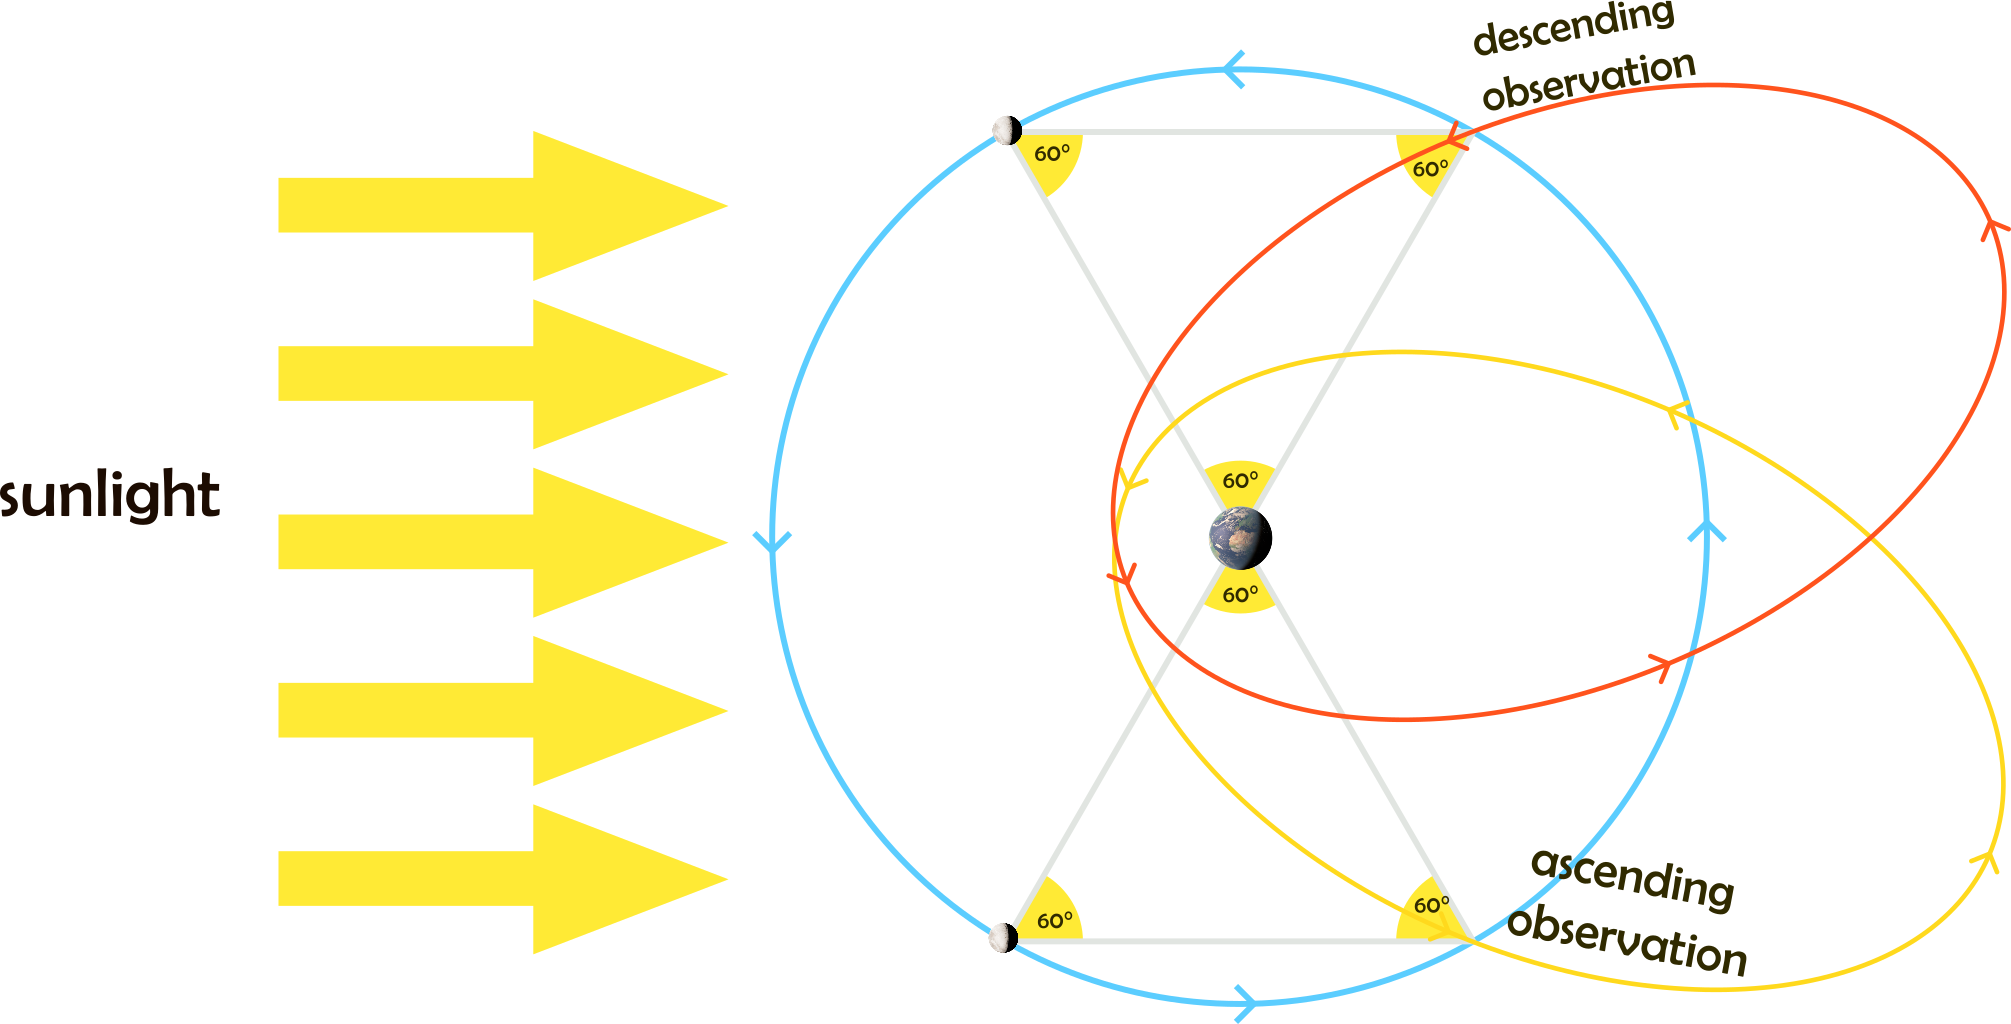
\includegraphics[width=10cm]{images/observations_main.png}
			\caption{keplerian orbit allowing to make long observation in a simplified model (fixed sun, circular orbit of the moon and observation zone distance equal to moon's orbit radius)}
		\end{figure}
		
		Using the solution that we found in 2D we can try to use it as an initial condition for 3D problems, the solution found with varying $\Omega$ value and considering the eccentricity of the Moon tend to show that there are always a solution near this point.
		
		A question that could arise from these observation can be about the importance of the device period over its speed in the observation zone. In other word, maybe it is better to force the device to match the speed of the observations zone instead of making it matcht the speed needed to get a fixed period.
		
		To answer this question i've made a quick test where for a set of position of the observation zone i've lanched the device with the same velocity vector as the observation zone, the result gave pretty high observation time of multiple hours, with the lowest possible time occuring when the observation time is near the Earth. This is not a problem as this kind of trajectory where not possible anyway because it require speed of around $1 km\cdot s^2$ at low altitudes.
		
		We can also see Three main peak, the first two are the one we find earlier with observations time of around 18 hours, and there a third one that is a little bit higher with observation time of around 24 hours.
		
		The fact that we make longer observation when the speed of of the observation zone match the speed of a circular orbit at its current position could be linked to the fact that the radial speed of the device start decreasing after crossing this altitude which could allow the device to make an oscilation around the observation point.
		
		about the last peak, the proximity of the observation from the Earth umbra and the fact that the corresponding device will have around the energy to escape the Earth sphere of influence (the speed of the Moon two time further than the Moon) make it not the better choice for reapeated observation.
		
		It could be an improvement of the method to drop the constraint on the speed norm and replace the two angle argument by a simple vector. Hovewer tests show worse result in most case when using only this algotithm to find solution while using this algorithm with the solution of the previous ones as initial condition barelly improve the solution.
		
		\subsection{finding initial guess}
		
		Now that we know where the observation roughly are we can create an algorithm that could easily find initial guess to find observation.
		
		as the speed of the device is constrained by its semi major axis (by the equation $\sqrt{\frac{2\mu}{R_s}-\frac{\mu}{a_l}}$), we just have to find the point where the observation zone speed matches the speed of the device.
			
		If we consider that the observation zone center is at the position of the point $P_{2x}$ we get :
		
		$$
		P_{2x}=R_l+\frac{D_{p2}}{D_{ts}}(R_l-R_s)
		$$
		where $D_{p2}$ is the distance between the moon and the point $P_{2x}$ where the moon is at the origin.
		the velocity of $P_{2x}$ is then straightforward to compute
		$$
		\dot{P_{2x}}=\dot{R_l}+\frac{D_{p2}}{D_{ts}}(\dot{R_l}-\dot{R_s})
		$$
		
		we can then get from this the following payoff formula :
		
		$$
		D_{obs}=\left(||\dot{P_{2x}}||-\sqrt{\frac{2\mu}{P_{2x}}-\frac{\mu}{a_l}}\right)^2
		$$  
		
		which is a one dimension equation depending of time only, which make it way easier to solve.
		
		\begin{figure}[h]
			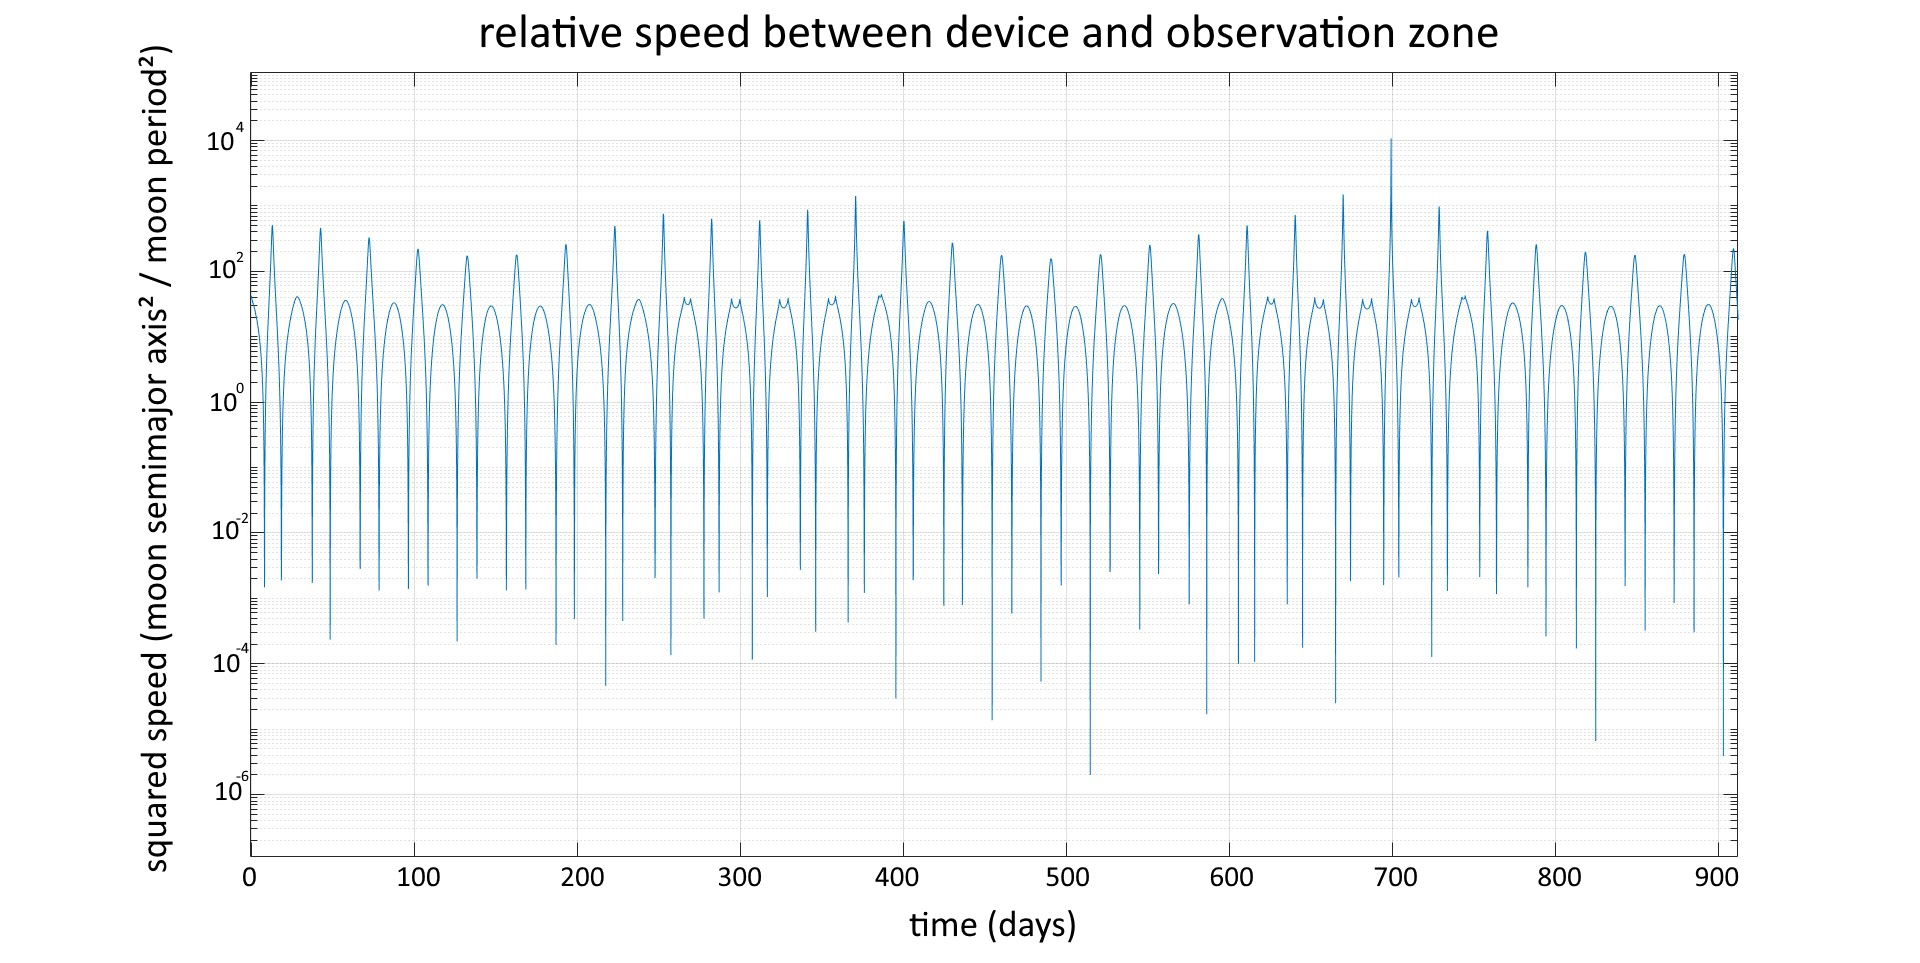
\includegraphics[width=12cm]{images/graph.jpg}
			\caption{relative speed between the device and the observation zone}
		\end{figure}
		
		we can see a periodic signal with a period equal to the synodic period of the device. A period is made of two local maximum corresponding to the time when the observation zone is the closest to Earth (the highest sharp peak)and when the observation zone is the farthest from Earth(the soft peak). There also two local minimum which correspond to the two points of interest. Theses minimum are around 5 days before and after the highest peak ($\frac{1}{6}$ time the synodic period exactly). 
		
		This configuration allow find estimate of time where the observation happen : 
		
		The first step consist of finding the high peak, the sharp peak would always be higher than 100 because of the high speed of the device near Earth and the soft peak would be always under 100 (because the speed difference can't be above $2\pi$ making the value of $D_{obs}$ smaller than $4\pi^2\approx 39$).
		
		this give us the following constrained problem:
		
		$$
		t^0=\arg \max D_{obs}(t)_{0\leq t ; D_{obs}(t)\geq100}
		$$
		
		by taking an initial guess at $t^0_0=0$ or finding the an estimation by hand should give us the first peak.
		
		we can then find every peak by solving the same problem with an initial guess of $t^n_0=t^{n-1}+P_{sy}$ where $t^{n-1}$ is the time of the last peak and $P_{sy}$ is the synodic period of the moon.
		
		we can then find the points of interests by finding the minimum	of the function $D_{obs}$ by taking the the following initial guess : 
		$$
		\begin{align}
			$O^{2n}_0&=t^n-\frac{P_{sy}}{6}\\
			$O^{2n+1}_0&=t^n+\frac{P_{sy}}{6}
		\end{align}
		$$ 
		
		A good thing about this method is that each problems (except the first one if we take $t^0_0=0$) can be easily sove with a simple gradient descent method. take also note that the first observation may be before 0 if the first peak happen at a time smaller than a sixth of the Synodic period.
		
		At last we can compute the vector $X_0$ for each of these time and then apply the real method to compute the best set of value for each observation.
		
		\begin{figure}[h]
			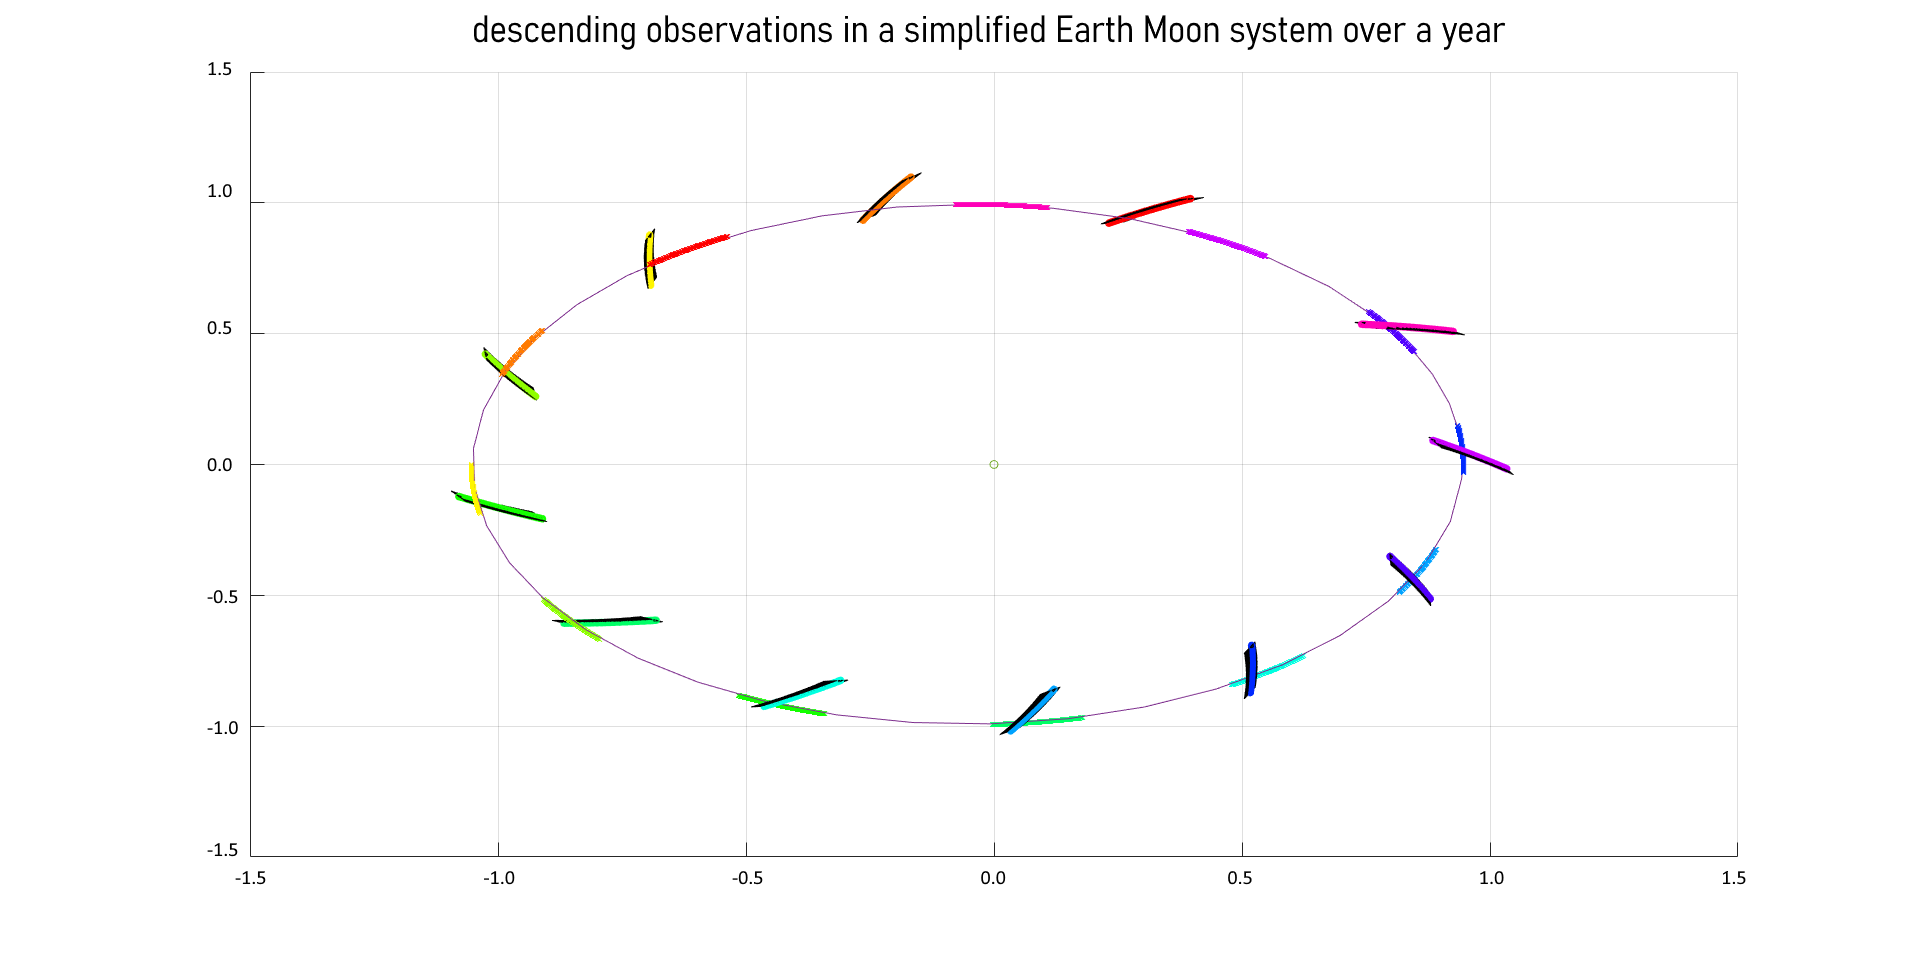
\includegraphics[width=1\textwidth]{images/observation_zone_year_scaled.png}
			\caption{descending observation zone over the course of one year, the position of the moon and the device is also added, the result show in this graph doesn't take in accout the variation of the moon orbit caused by the sun}
		\end{figure}
		
		the problem of this simplified model is that we fixed the period of the device at the period of the Moon which was an hypothesis to reduce thrust needed between transfert but not realy an argument for maximizing the observation time.
		
		in fact I've noticed that observation time were higher when the period of the device was slightly reduced (around 0.92 Lunar period). I didn't manage to find the exact cause of this pheonomenon, i think a better model than this one could be around...
		
		For the rest of this article the value of the device period was fixed at 0.92 as it give longer observation time. 
		
		\subsection{impact of alpha on the observation time}
		
		i've made a few test of the algorithm with mulitple value of alpha. I've fetch all observations happening between january 4th of 2025 and january 2nd of 2027. here's the observations time we got from theses:  
		\begin{center}
			\begin{tabular}{||c||c c c c c||} 
				\hline
				alpha & 10\% & 5\% & 2\% &1\% & 0.5\% \\ [0.5ex] 
				\hline\hline
				maximum & 28h01min & 21h26min & 15h02min &11h31min & 8h46min \\ 
				\hline
				minimum & 23h30min & 18h00min & 12h42min &9h42min& 6h34min \\
				\hline
				median & 25h26min & 19h29min & 13h40min &10h30min& 8h06min\\
				\hline
				mean & 25h35min & 19h35min & 13h47min &10h33min& 8h04min\\ 
				\hline
			\end{tabular}
		\end{center}
		
		the result with the observation zone at 5\% will be used in the rest of the article.
		
		\section{low thrust transfert}
			
			\subsection{low thrust model}
			
			we want to move from a point $R_i$ at time $t_i$ to a point $R_f$ at time $t_f$ with initial velocity $V_i$ and final velocity $V_f$.
			
			the device can be control with a low thrust engine that can generate an acceleration of maximum magnitude $A_{max}$ in any direction, as the final objective is to use a solar sail, the variation of mass is neglected.
			
			the passive dynamic of the device is the following : 
			$$
			\begin{bmatrix}
				\dot{r}\\
				\dot{v}
			\end{bmatrix} =\begin{bmatrix}
				v\\
				\sum\limits _{\beta \in B }\frac{\mu _{\beta }}{\| r_{\beta } -r\| ^{3}}( r_{\beta } -r)
			\end{bmatrix}
			$$
			
			where $B$ is the set of every bodies that attract the device (for now the two body are The Earth and the Moon). the dynamics of the bodies must be computed before (we suppose that the device does not influence the dynamics of the system).
			
			the acceleration of the thruster can be take in account by adding a vector the equations of speed : \\
			
			$$
			f(x,u)=\dot{x}=
			\begin{bmatrix}
				\dot{r}\\
				\dot{v}
			\end{bmatrix}
			=\begin{bmatrix}
				v\\
				u+\sum\limits _{\beta \in B }\frac{\mu _{\beta }}{\| r_{\beta } -r\| ^{3}}( r_{\beta } -r)
			\end{bmatrix}
			$$
			
			we want to minimize the $\Delta_v$ of the transfert, so the running payoff is :
			$$
			r(x,u)=-\|u\|
			$$ 
			
			we also want to be at the right position and velocity at the time $t_f$ so the terminal payoff is :
			
			$$
			g(x(t_f))=-(r(t_f)-R_f)^2-(v(t_f)-V_f)^2
			$$
			
			we get the following hamiltonian :
			
			$$
			H(x,p,u)=\begin{bmatrix}
				v\\
				u+\sum\limits _{\beta \in B }\frac{\mu _{\beta }}{\| r_{\beta } -r\| ^{3}}( r_{\beta } -r)
			\end{bmatrix}^t\cdot p-\|u\|
			$$
			
			using the Pontryagin maximum principle theorem we can compute the differential of $p=\begin{bmatrix}p_r\\p_v\end{bmatrix}$
			
			$$
			\begin{align}
				\dot{p}=&-\nabla _{x}H\\
				=&-\begin{bmatrix}
					0 & I_3\\
					\sum\limits _{\beta \in B }\frac{\mu _{\beta }}{\| r_{\beta } -r\| ^{3}}\left(\frac{3( r_{\beta } -r) \cdot ( r_{\beta } -r)^{t}}{\| r_{\beta } -r\| ^{2}} -I_3\right) & 0
				\end{bmatrix}^{t} \cdot p\\
				=&\begin{bmatrix}
					\sum\limits _{\beta \in B }\frac{\mu _{\beta }}{\| r_{\beta } -r\| ^{3}}\left(I_3-\frac{3( r_{\beta } -r) \cdot ( r_{\beta } -r)^{t}}{\| r_{\beta } -r\| ^{2}} \right)\cdot p_v\\
					-p_r
				\end{bmatrix}
			\end{align}
			$$
			
			we know that $\forall t$ , $u=\arg\max_{u\in B(0,A_{max})}H(x,p,u)$. We can rewrite the hamiltonian as follow : 
			$$
			\begin{align}
				H(x,p,u)=&C(x,p)+u\cdot p_v-\|u\| \\
				=&C(x,p)+\|u\|(\|p_v\|\cos(\alpha_{\widehat{up_v}})-1)
			\end{align}
			$$ 
			
			with this form we can easily conclude that 
			$$
			\begin{cases}
				\| u\| =A_{max} & \text{if } \|p_v\|\cos(\alpha_{\widehat{up_v}})\ge1\\
				\| u\| =0 & \text{else}
			\end{cases}
			$$
			
			we can then observe that $\|p_v\|\cos(\alpha_{\widehat{ap_v}})$ cannot be greater than $1$ if $\|p_v\| < 1$. Also if $\|p_v\| \ge 1$, it is obvious that taking $\alpha_{\widehat{up_v}}=0$ (i.e. $u$ and $p_v$ are collinear) maximize the factor $\|p_v\|\cos(\alpha_{\widehat{uap_v}})$. So we can conclude the following formula :
			
			$$
			\begin{cases}
				 u =A_{max}\widehat{p_v} & \text{if }\|p_v\| \ge 1\\
				 u =0 & \text{else}
			\end{cases}
			$$
			
			to solve the problem numerically, we then just have to find the correct value $p_i$ so the terminal value of $x$ correspond to the target value.
			
			\section{result low thrust}
				\\
			to compute the solution, i've used the julia library : OptimalControl,
			
			the starting point of the device is the exting point where of starting observation and the ending point is the enter point of the ending observation.
			
			To simplify the next explication i will separate the observations into two category : the ascending observations and the descending observation. The descending observations are observations happening when the moon is around it last crescent, in this configuration the device must aproach Earth to make an observation. The ascending observation is the opposite, happening when the moon is around its first crescent and needed the device to moving away from earth.
			
			\subsection{observation}
			The algorithm had a lot of struggle to find an optimum for moving to two adjacent observations, which was excpected as the two orbit of adjacent optimum are very different and the time interval is small meaning that important $\Delta_v$ are needed to move from the starting point to the ending point. hovewer the algorithm find solution for transition between ascending observation and between descending observation. This was also excpected as the starting and objective orbit are very similar with the main difference being only a rotation of $\frac{P_{moon}}{P_{sol}}2\pi $ rad caused by the movement of the sun.
			\\ \\
			for 1 in 2 transfert, the maximum acceleration found was betweeen $170 \mu{N}\cdot\text{Kg}$ and $200 \mu{N}\cdot\text{Kg}$ which is around the acceleration we can get from electric engine but not from solar sail.
		
			there are also another type of transfert that caught my interest, it is transfert from descending observation to ascending observation (1 in 3 transfert starting from descending observation) which seem to be very easy to do with maximum acceleration ranging from  $50 \mu{N}\cdot\text{Kg}$ to $95 \mu{N}\cdot\text{Kg}$. It truned out that the angle between an descending orbit and a ascending orbit orbit is around the same length of the angle describe by the movement of the sun in $\frac{4}{3}$ of the moon synodic period, this mean that the starting and ending orbit in such transfert are almost the same with the only main task being to change the true anomaly. This transferts could look like they are a good alternative to reduce maximum acceleration during transfert but the problem is that once we reached the descending observation, we have to make a transfert from ascending to descending and in this case the situation is reverse with the angles being added and not substracted, causing high maximum acceleration.
			\\ \\
			In fact making fewer observation doesn't seem to reduce the maximum acceleration needed or ascending the $\Delta_{V}$ which could look counter intuitive at first glance but is not when we think aboout the fact that orbits become increasingly different from each other with time. This mean that there shold be some kind of minimum power needed for making observations which must be around the amount of power needed to rotate the observation orbit by $360^\circ$ every year. considering the result that we have now, the device should be able to deliver a delta V of around $5Km\cdot s^{-1} $ every year, which is not that far of what solar sail could do , but we don't take in account here the constraint given by solar sail that will likely increase this value.
			
			
			
			 with this said it is possible to jump a lot of observations to the point that we don't need to rotate the orbit all around the Earth. Like with the obvious example of making an observation every year, when the sun is roughly at the same place relative to the Earth-Moon system. But the counter part is that we will be making way less observations ... at most one every 6 mouths. 
			
			here some illustration to better understand the different possible transfert (note that theses graphics show approximative position of observations orbits and are not made from real data):
			
			\begin{figure}[h]
				\includegraphics[width=0.5\textwidth]{images/1in2obs.png}
				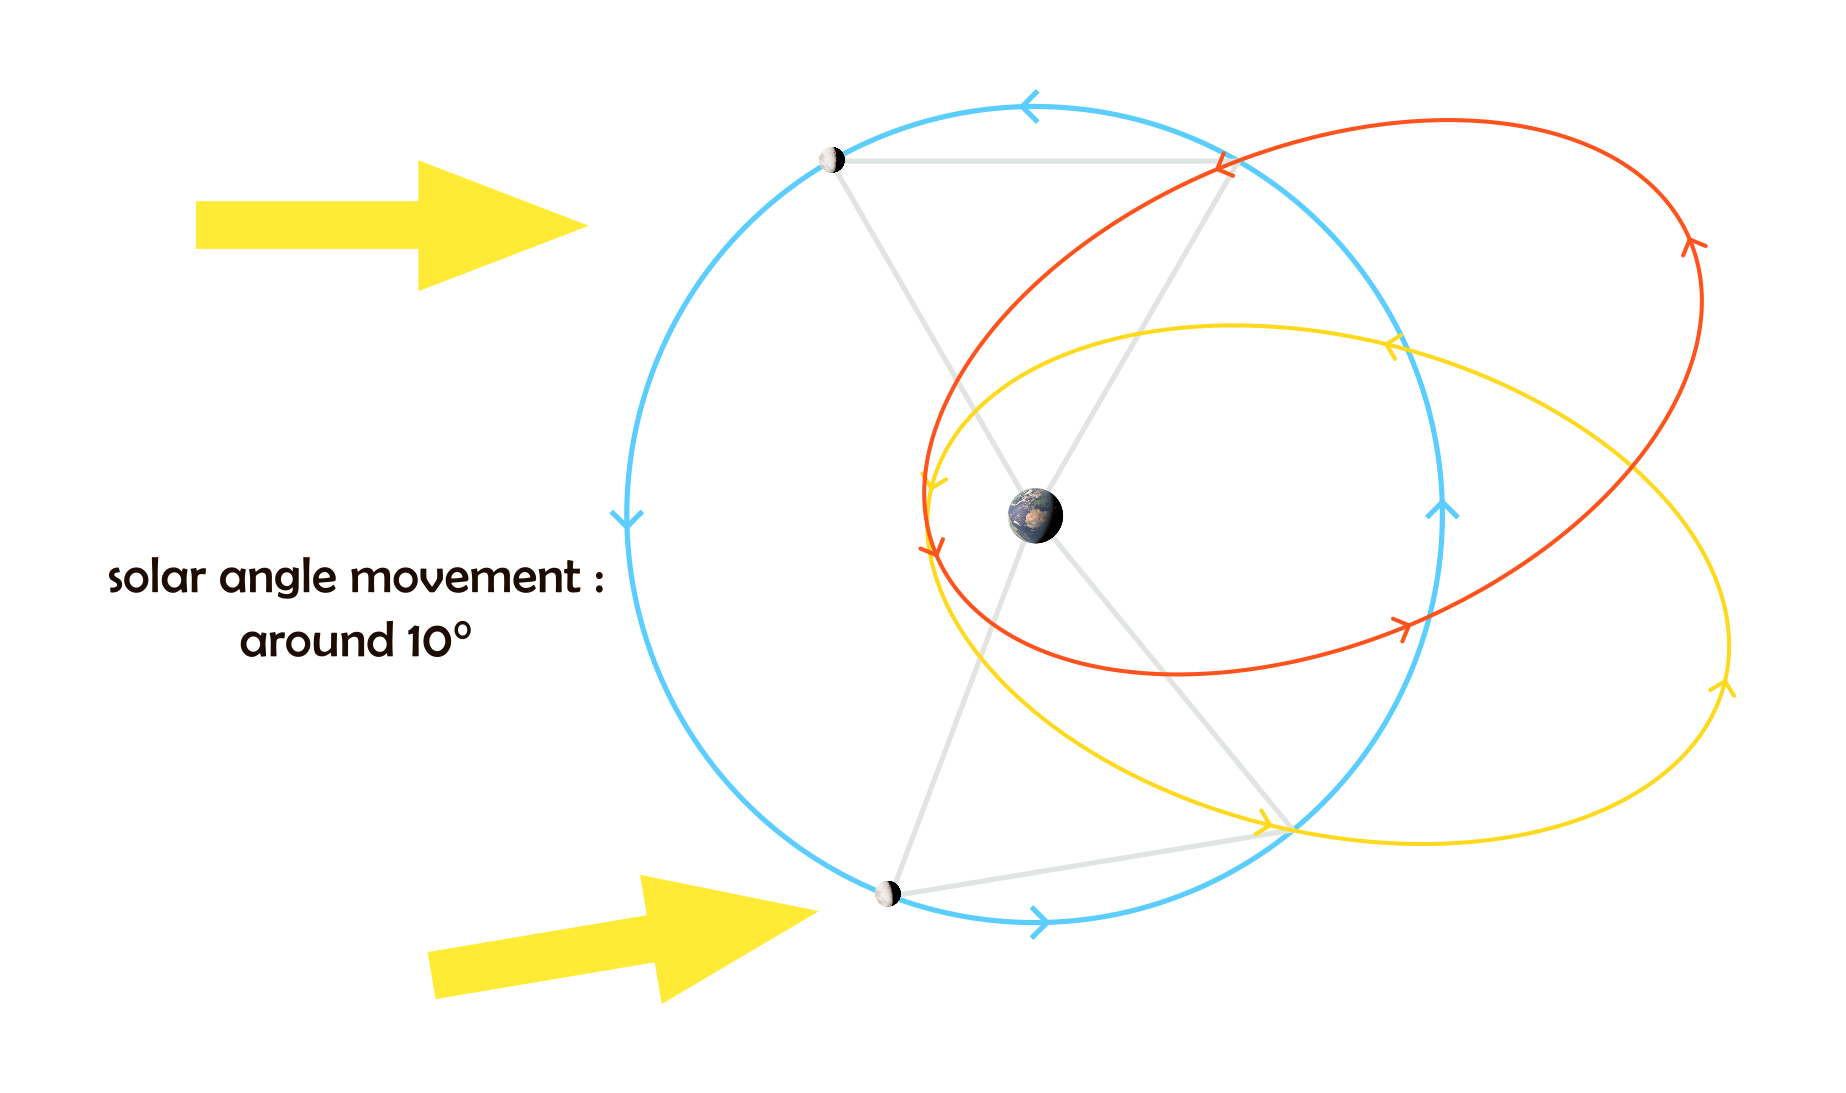
\includegraphics[width=0.5\textwidth]{images/odd_to_even.png}
				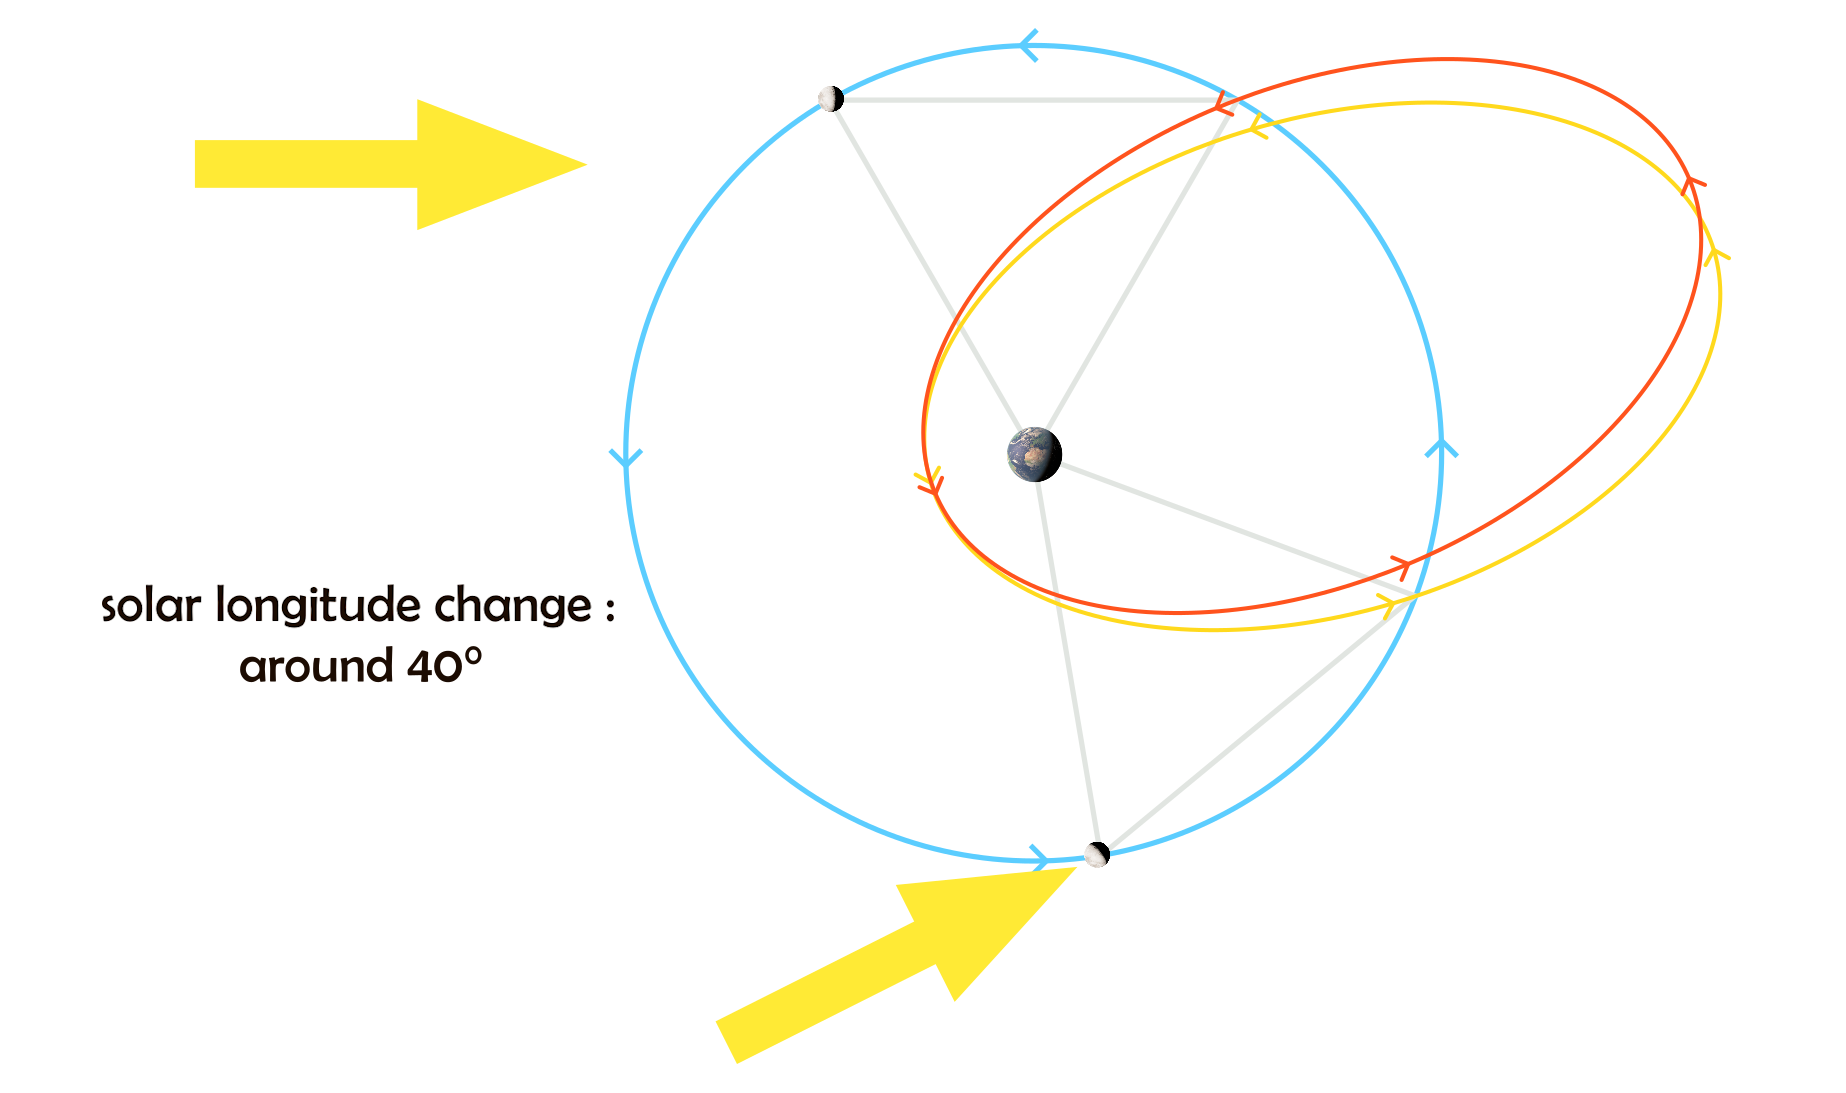
\includegraphics[width=0.5\textwidth]{images/1in3_obs.png}
				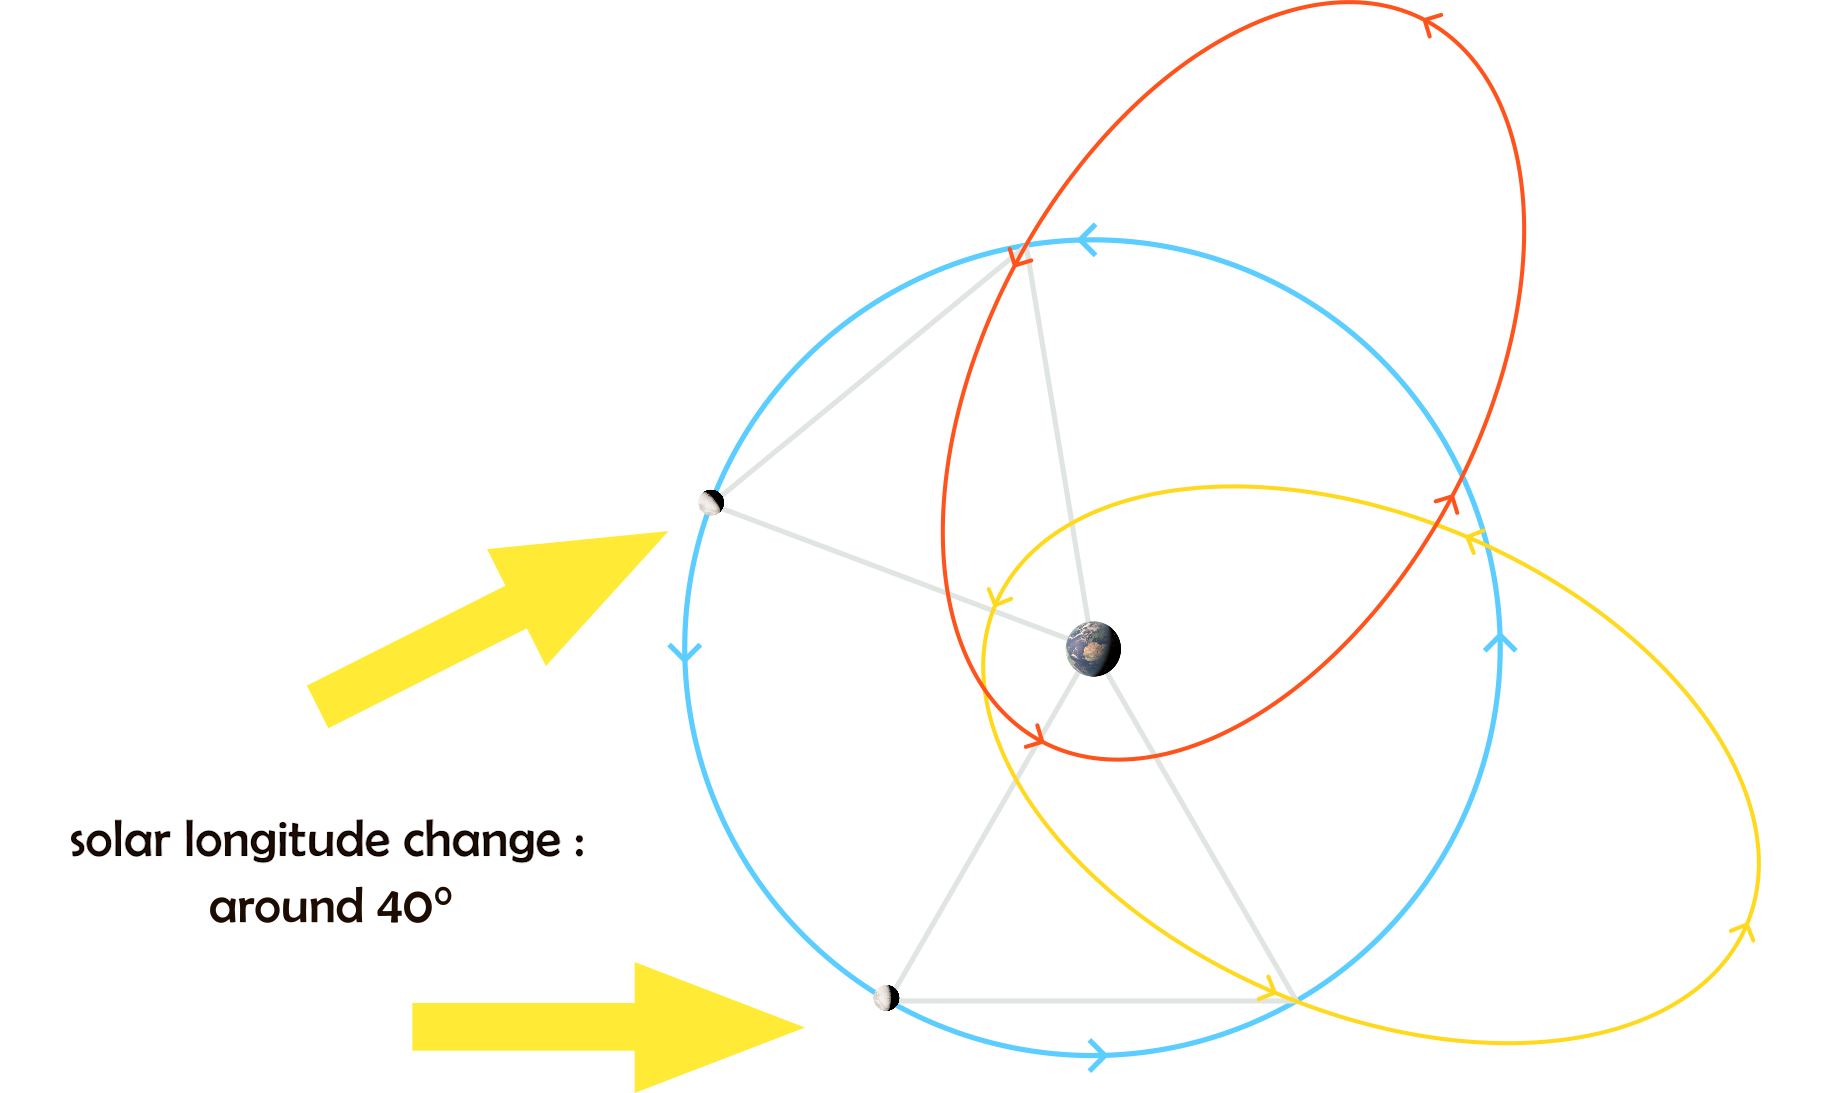
\includegraphics[width=0.5\textwidth]{images/1in3_bad.png}
			\end{figure}
			
			here we can see that the top left transfert (descending observations to descending observation) is relatively easy to do with having to rotate a little bit the orbit in around 29 days. Hovewer, making a transfert from and descending to ascending observations like in the top right  would need the device to make a bigger change in orbit in abour 3 times less time. moving from ascending to descending observation will be even harder as the orbit move apart from each other instead of getting closer.
			
			the bottom left illustration show the easiest transfert where the sun magnitude change compensate almost exactly the angle between descending and ascending observation making the transfert only a question of changing the true anomaly.
			
			like for the two other transfert, moving from ascending to descending observation are harder as the sun magnitude change cumulate instead of cancelling the angle between descending and ascending observation. 
			
			
			
			\subsection{scenario with solar sail}
			
			Using solar sails with their actual performance level (around $50\mu{m}\cdot\text{s}^2$) won't allow to make a lot of observations, with the only plausible scenario that far could be to make an descending observation follow by a ascending observation 40 days later taking advantage of the low maximum acceleration of these transfert. Then spend multiples mounths aligning for another descending observations and repeating the process in a cycle of at least 8 mouths which is still way better than what we could do on Earth. But ascending this scenario may be infeasible once the additional sail constraint on the control are added.
			
			another possibility could be about the third observation that i had consider to too impractical to be usefull at first but may give better result when making only a few observation per years.
			
			\subsection{scenario with electric propulsion}	
			\\ \\
			What look like the best scenario at this point would be to put two devices capable of delivering acceleration of the order of $300\mu{m}\cdot\text{s}^2$, one for the descending observation and one for the ascending observation. This would allow to attends every observations which mean that we will be able to observe the solar corona around $2.8\%$ of the mission time with ascending the possibility of observing the sun and the sun corrona at the same time if one device aim at the sun during the observation of the other device.
			
			To get more data about these scenario i've added the equation of mass to the dynamics of the system. for the next result i've use the following theoretical spacecraft : 
			
			the device has $50Kg$ of payload with $40Kg$ of fuel, the engine used is the RIT-10 evo from 
			 
	
		\end{document}